% !TeX root = RJwrapper.tex
\title{Predicting Motor Vehicle Collisions in New York City}
\author{by Alex Fung, Viswesh Krishnamurthy, Tony Lee, Patrick Osborne}

\maketitle


\begin{Schunk}
\begin{Soutput}
#> [1] 56000
\end{Soutput}
\end{Schunk}

\begin{Schunk}
\begin{Sinput}
#code below IS shown in final document
\end{Sinput}
\end{Schunk}

\hypertarget{abstract}{%
\subsection{Abstract}\label{abstract}}

Technological progress in the world has unarguably improved the quality
of life for the average person in many ways. The age of the automobile
has shaped the way in which work, play and live our lives. Roadways,
buildings, cities and entire countries have been designed to accommodate
motor vehicles. As automobile technology has advanced making cars faster
and capable of more advanced maneuvers, so has our concern with the
safety of these vehicles. Entire disciplines such as traffic management
are devoted to optimizing numerous factors to ensure the safe and
efficient movement of people and goods. As we move into the age of data,
all stakeholders in the automobile industry must effectively collect and
utilize the wealth of information available to better meet their goals
if progress is to continue. In this project, we take the position of a
law enforcement agency, the New York City Police Department, as they
seek to best utilize their resources in the context of responding to
traffic collisions in the city.

\hypertarget{background}{%
\subsection{Background}\label{background}}

At the end of 2017 in New York City, there were 1,923,041 cars
registered to residents of the city.
(\url{https://nyc.streetsblog.org/2018/10/03/car-ownership-continues-to-rise-under-mayor-de-blasio/})
This already-significant number does not include the heavy flow of
vehicles of those who visit the city or are simply passing through. By
contrast, the New York City Police Department (NYPD) budgets for a
headcount of 35,822 uniformed officers
(\url{http://council.nyc.gov/budget/wp-content/uploads/sites/54/2017/03/056-NYPD.pdf}
- page 4), distributed across 77 police precincts (geographic divisions
of the city). On-duty officers/traffic enforcement agents are allocated
to each precinct to enforce traffic laws and handle emergency and
administrative response to traffic incidents (such as collisions). NYC
has been collecting traffic data, including specific data on vehicle
collisions since 2014 to support ``Vision Zero'' , a traffic safety
initiative which has the goal of eliminating traffic fatalities.
(\url{https://data.cityofnewyork.us/Public-Safety/Motor-Vehicle-Collisions-Crashes/h9gi-nx95/data})

\hypertarget{objective}{%
\subsection{Objective}\label{objective}}

The objective of our analysis is to develop a supervised, prediction
model using Machine Learning techniques and the CRISP-DM framework (cite
textbook) on the available collision data to predict whether there will
be a collision in a specified police precinct at a specified time. The
intent of predicting this data is to inform the NYPD's optimal
assignment of limited officers and resources across the 77 police
precincts.

\hypertarget{data-analysis}{%
\subsection{Data Analysis}\label{data-analysis}}

The data set that supports this analysis is sourced from the NYC Open
Data project. The title of the data set is ``Motor Vehicle Collisions --
Crashes''. It contains entries for every collision recorded within New
York City limits by NYPD agents beginning July 1st, 2012 up to the
present day. There are approximately 1.65 million entries in the data
set.

\hypertarget{data-dictionary}{%
\subsection{Data Dictionary}\label{data-dictionary}}

Data dictionary sourced from
\url{https://data.cityofnewyork.us/Public-Safety/Motor-Vehicle-Collisions-Crashes/h9gi-nx95/data}
- ``MVCollisionsDataDictionary\_20190813\_ERD.xlsx''.

\begin{table}

\caption{\label{tab:data-dictionary}Data Dictionary - Motor Vehicle Collisions – Crashes}
\centering
\begin{tabular}[t]{l|l}
\hline
Feature & Feature.Description\\
\hline
COLLISION\_ID & Unique record code generated by system\\
\hline
ACCIDENT\_DATE & Occurrence date of collision\\
\hline
ACCIDENT\_TIME & Occurrence time of collision\\
\hline
BOROUGH & Borough where collision occurred\\
\hline
ZIP CODE & Postal code of incident occurrence\\
\hline
LATITUDE & Latitude coordinate for Global Coordinate System, WGS 1984\\
\hline
LONGITUDE & Longitude coordinate for Global Coordinate System, WGS 1984\\
\hline
LOCATION & Latitude , Longitude pair\\
\hline
ON STREET NAME & Street on which the collision occurred\\
\hline
CROSS STREET NAME & Nearest cross street to the collision\\
\hline
OFF STREET NAME & Street address if known\\
\hline
NUMBER OF PERSONS INJURED & Number of persons injured\\
\hline
NUMBER OF PERSONS KILLED & Number of persons killed\\
\hline
NUMBER OF PEDESTRIANS INJURED & Number of pedestrians injured\\
\hline
NUMBER OF PEDESTRIANS KILLED & Number of pedestrians killed\\
\hline
NUMBER OF CYCLIST INJURED & Number of cyclists injured\\
\hline
NUMBER OF CYCLIST KILLED & Number of cyclists killed\\
\hline
NUMBER OF MOTORIST INJURED & Number of vehicle occupants injured\\
\hline
NUMBER OF MOTORIST KILLED & Number of vehicle occupants killed\\
\hline
CONTRIBUTING FACTOR VEHICLE 1 & Factors contributing to the collision for designated vehicle\\
\hline
CONTRIBUTING FACTOR VEHICLE 2 & Factors contributing to the collision for designated vehicle\\
\hline
CONTRIBUTING FACTOR VEHICLE 3 & Factors contributing to the collision for designated vehicle\\
\hline
CONTRIBUTING FACTOR VEHICLE 4 & Factors contributing to the collision for designated vehicle\\
\hline
CONTRIBUTING FACTOR VEHICLE 5 & Factors contributing to the collision for designated vehicle\\
\hline
VEHICLE TYPE CODE 1 & Type of vehicle based on the selected vehicle category\\
\hline
VEHICLE TYPE CODE 2 & Type of vehicle based on the selected vehicle category\\
\hline
VEHICLE TYPE CODE 3 & Type of vehicle based on the selected vehicle category\\
\hline
VEHICLE TYPE CODE 4 & Type of vehicle based on the selected vehicle category\\
\hline
VEHICLE TYPE CODE 5 & Type of vehicle based on the selected vehicle category\\
\hline
\end{tabular}
\end{table}

\newpage

\hypertarget{initial-data-exploration-and-cleaning}{%
\subsection{Initial Data Exploration and
Cleaning}\label{initial-data-exploration-and-cleaning}}

{[}SUMMARY OF DATA INSERT TEXT{]}

\scalebox{0.6}{
\begin{tabular}{llllll}
  \hline
     CRASH.DATE &   CRASH.TIME &          BOROUGH &    ZIP.CODE &    LATITUDE &   LONGITUDE \\ 
  \hline
01/21/2014:   1161   & 16:00  :  24074   &              :499865   & Min.   :10000   & Min.   : 0.00   & Min.   :-201.36   \\ 
  11/15/2018:   1065   & 17:00  :  23613   & BRONX        :160097   & 1st Qu.:10304   & 1st Qu.:40.67   & 1st Qu.: -73.98   \\ 
  12/15/2017:    999   & 15:00  :  23171   & BROOKLYN     :355543   & Median :11206   & Median :40.72   & Median : -73.93   \\ 
  05/19/2017:    974   & 18:00  :  21767   & MANHATTAN    :273153   & Mean   :10828   & Mean   :40.69   & Mean   : -73.87   \\ 
  01/18/2015:    961   & 14:00  :  21258   & QUEENS       :305510   & 3rd Qu.:11237   & 3rd Qu.:40.77   & 3rd Qu.: -73.87   \\ 
  02/03/2014:    960   & 13:00  :  19732   & STATEN ISLAND: 49124   & Max.   :11697   & Max.   :43.34   & Max.   :   0.00   \\ 
  (Other)   :1637172   & (Other):1509677   &  & NA's   :500110   & NA's   :199425   & NA's   :199425   \\ 
   \hline
\end{tabular}
}
\scalebox{0.6}{
\begin{tabular}{llll}
  \hline
                          LOCATION &                          ON.STREET.NAME &                        CROSS.STREET.NAME &                                 OFF.STREET.NAME \\ 
  \hline
                              : 199425   &                                 : 323553   &                                 : 555996   &                                         :1411905   \\ 
  POINT (0 0)                   :   1113   & BROADWAY                        :  16258   & 3 AVENUE                        :   9846   & 772       EDGEWATER ROAD                :    375   \\ 
  POINT (-74.038086 40.608757)  :    670   & ATLANTIC AVENUE                 :  14401   & BROADWAY                        :   9685   & 110-00    ROCKAWAY BOULEVARD            :    244   \\ 
  POINT (-73.9845292 40.6960346):    586   & 3 AVENUE                        :  11761   & 2 AVENUE                        :   8425   & 2800      VICTORY BOULEVARD             :    221   \\ 
  POINT (-73.98453 40.696033)   :    574   & NORTHERN BOULEVARD              :  11460   & 5 AVENUE                        :   7052   &                                         :    183   \\ 
  POINT (-73.91282 40.861862)   :    545   & BELT PARKWAY                    :  11302   & 7 AVENUE                        :   6634   & 2100      BARTOW AVENUE                 :    158   \\ 
  (Other)                       :1440379   & (Other)                         :1254557   & (Other)                         :1045654   & (Other)                                 : 230206   \\ 
   \hline
\end{tabular}
}
\scalebox{0.6}{
\begin{tabular}{llll}
  \hline
NUMBER.OF.PERSONS.INJURED & NUMBER.OF.PERSONS.KILLED & NUMBER.OF.PEDESTRIANS.INJURED & NUMBER.OF.PEDESTRIANS.KILLED \\ 
  \hline
Min.   : 0.0000   & Min.   :0.000000   & Min.   : 0.00000   & Min.   :0.000000   \\ 
  1st Qu.: 0.0000   & 1st Qu.:0.000000   & 1st Qu.: 0.00000   & 1st Qu.:0.000000   \\ 
  Median : 0.0000   & Median :0.000000   & Median : 0.00000   & Median :0.000000   \\ 
  Mean   : 0.2634   & Mean   :0.001174   & Mean   : 0.05092   & Mean   :0.000641   \\ 
  3rd Qu.: 0.0000   & 3rd Qu.:0.000000   & 3rd Qu.: 0.00000   & 3rd Qu.:0.000000   \\ 
  Max.   :43.0000   & Max.   :8.000000   & Max.   :27.00000   & Max.   :6.000000   \\ 
  NA's   :17   & NA's   :31   &  &  \\ 
   \hline
\end{tabular}
}
\scalebox{0.6}{
\begin{tabular}{llll}
  \hline
NUMBER.OF.CYCLIST.INJURED & NUMBER.OF.CYCLIST.KILLED & NUMBER.OF.MOTORIST.INJURED & NUMBER.OF.MOTORIST.KILLED \\ 
  \hline
Min.   :0.00000   & Min.   :0.00e+00   & Min.   : 0.000   & Min.   :0.000000   \\ 
  1st Qu.:0.00000   & 1st Qu.:0.00e+00   & 1st Qu.: 0.000   & 1st Qu.:0.000000   \\ 
  Median :0.00000   & Median :0.00e+00   & Median : 0.000   & Median :0.000000   \\ 
  Mean   :0.02062   & Mean   :8.34e-05   & Mean   : 0.192   & Mean   :0.000452   \\ 
  3rd Qu.:0.00000   & 3rd Qu.:0.00e+00   & 3rd Qu.: 0.000   & 3rd Qu.:0.000000   \\ 
  Max.   :4.00000   & Max.   :2.00e+00   & Max.   :43.000   & Max.   :5.000000   \\ 
   \hline
\end{tabular}
}
\scalebox{0.6}{
\begin{tabular}{llll}
  \hline
               CONTRIBUTING.FACTOR.VEHICLE.1 &                CONTRIBUTING.FACTOR.VEHICLE.2 &                CONTRIBUTING.FACTOR.VEHICLE.3 &                CONTRIBUTING.FACTOR.VEHICLE.4 \\ 
  \hline
Unspecified                   :599544   & Unspecified                   :1193786   &                               :1536917   &                               :1621113   \\ 
  Driver Inattention/Distraction:308381   &                               : 222550   & Unspecified                   :  98931   & Unspecified                   :  20912   \\ 
  Failure to Yield Right-of-Way : 94090   & Driver Inattention/Distraction:  75420   & Other Vehicular               :   1949   & Other Vehicular               :    364   \\ 
  Following Too Closely         : 82937   & Other Vehicular               :  27258   & Driver Inattention/Distraction:   1424   & Following Too Closely         :    237   \\ 
  Backing Unsafely              : 62951   & Failure to Yield Right-of-Way :  14284   & Following Too Closely         :   1298   & Driver Inattention/Distraction:    175   \\ 
  Other Vehicular               : 52108   & Following Too Closely         :  14009   & Fatigued/Drowsy               :    853   & Fatigued/Drowsy               :    170   \\ 
  (Other)                       :443281   & (Other)                       :  95985   & (Other)                       :   1920   & (Other)                       :    321   \\ 
   \hline
\end{tabular}
}
\scalebox{0.6}{
\begin{tabular}{llll}
  \hline
               CONTRIBUTING.FACTOR.VEHICLE.5 &  COLLISION\_ID &                          VEHICLE.TYPE.CODE.1 &                          VEHICLE.TYPE.CODE.2 \\ 
  \hline
                              :1637609   & Min.   :     22   & PASSENGER VEHICLE                  :715236   & PASSENGER VEHICLE                  :537550   \\ 
  Unspecified                   :   5361   & 1st Qu.:1038275   & SPORT UTILITY / STATION WAGON      :313500   &                                    :273620   \\ 
  Other Vehicular               :     96   & Median :3457776   & Sedan                              :172288   & SPORT UTILITY / STATION WAGON      :237846   \\ 
  Following Too Closely         :     51   & Mean   :2808228   & Station Wagon/Sport Utility Vehicle:140852   & Sedan                              :128269   \\ 
  Fatigued/Drowsy               :     41   & 3rd Qu.:3868829   & TAXI                               : 50670   & Station Wagon/Sport Utility Vehicle:108877   \\ 
  Driver Inattention/Distraction:     40   & Max.   :4280357   & VAN                                : 26540   & (Other)                            :357127   \\ 
  (Other)                       :     94   &  & (Other)                            :224206   & NA's                               :     3   \\ 
   \hline
\end{tabular}
}
\scalebox{0.6}{
\begin{tabular}{llll}
  \hline
                         VEHICLE.TYPE.CODE.2 &                          VEHICLE.TYPE.CODE.3 &                          VEHICLE.TYPE.CODE.4 &                          VEHICLE.TYPE.CODE.5 \\ 
  \hline
PASSENGER VEHICLE                  :537550   &                                    :1507965   &                                    :1593350   &                                    :1632527   \\ 
                                     :273620   & PASSENGER VEHICLE                  :  63655   & PASSENGER VEHICLE                  :  24743   & PASSENGER VEHICLE                  :   5476   \\ 
  SPORT UTILITY / STATION WAGON      :237846   & SPORT UTILITY / STATION WAGON      :  33161   & SPORT UTILITY / STATION WAGON      :  14375   & SPORT UTILITY / STATION WAGON      :   3138   \\ 
  Sedan                              :128269   & Sedan                              :  11698   & Sedan                              :   2598   & Sedan                              :    668   \\ 
  Station Wagon/Sport Utility Vehicle:108877   & Station Wagon/Sport Utility Vehicle:   9730   & Station Wagon/Sport Utility Vehicle:   2102   & Station Wagon/Sport Utility Vehicle:    548   \\ 
  (Other)                            :357127   & UNKNOWN                            :   3285   & TAXI                               :   1681   & TAXI                               :    246   \\ 
  NA's                               :     3   & (Other)                            :  13798   & (Other)                            :   4443   & (Other)                            :    689   \\ 
   \hline
\end{tabular}
}

Based on what we know about the data set from the specifications at NYC
Open Data and the data dictionary, we have decided to perform some
initial cleaning steps.

Our analytics problem is to predict whether there will be a collision at
a specific time (time including a time of the day, day of the year and
calendar year). In this context, we will first look at the
``CRASH.DATE'' graph. Thinking about the scheduling of police resource,
we assume that this happens in advance, on a hour-by-hour and day-by-day
basis. We assume that resources are not scheduled on a year-by-year
basis due to uncertainty in staffing, budget, etc. We therefore examine
the data to see whether we should include the year at all. Including the
year would treat the data set as a time-series, years ranging from
2012-2020. Alternatively, we could drop the year and group all
occurrences on the same day in the same bin, possibly enhancing our
prediction.

To decide, we plot the dates and look for trends. If trends repeat
annually, we will drop the year as this trend will be preserved when we
combine. If the trend does not repeat annually (extends over the whole
range of dates) then we will not combine year as we will lose this
information when dropping year.

\begin{Schunk}
\begin{figure}

{\centering 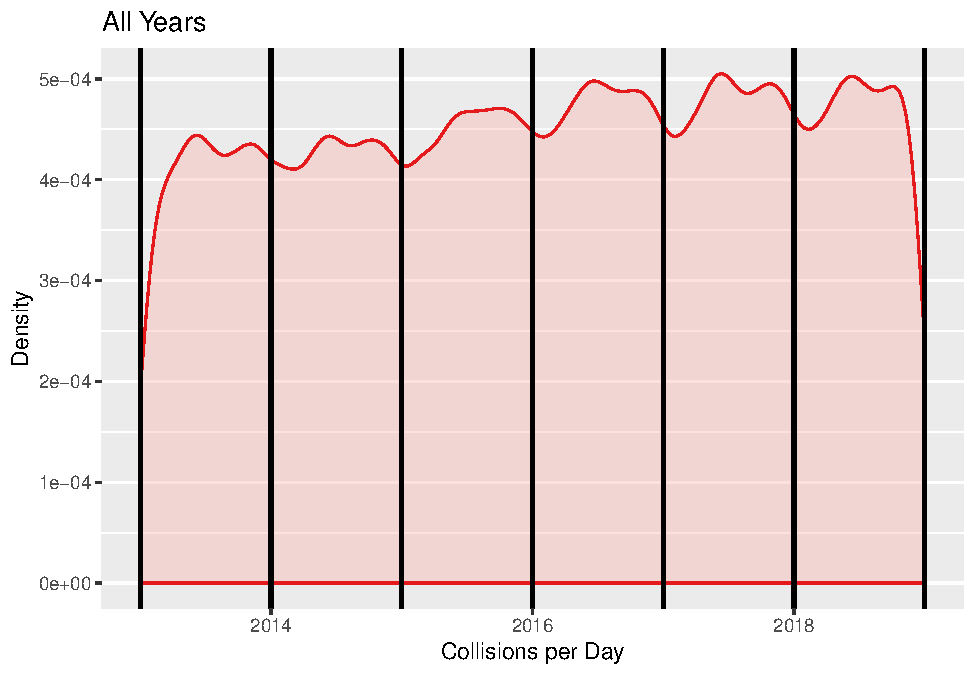
\includegraphics{RMarkdown-Group_10-Assignment_1_files/figure-latex/unnamed-chunk-4-1} 

}

\caption[Collisions per Day - All Years]{Collisions per Day - All Years}\label{fig:unnamed-chunk-4}
\end{figure}
\end{Schunk}

The vertical black lines in the ``All Years'' plot represent the start
of each year. As you can see from the plot, there is a noticeable
repeating trend in each year (between the black lines) with a decrease
in collisions at the start of each year, followed by various other
increase/decreases. As we are more interested in capturing this
repeating annual trend than year-over-year changes, we will combine all
data into a representation of one year. Additionally, we will drop years
2012 and 2020 (the first and last years in the data set) to avoid
over/under-representing specific months in the combined-year data set.
This leaves us with the ``Years Combined'' data set plotted below.

We use the following code to keep only data in 2013 onwards and in prior
to 2020, as mentioned.

\begin{Schunk}
\begin{Sinput}
raw_crash_dates_df <- raw_crash_dates_df[raw_crash_dates_df$raw_crash_dates > "2013-01-01", ]
raw_crash_dates_df <- raw_crash_dates_df[raw_crash_dates_df$raw_crash_dates < "2020-01-01", ]
\end{Sinput}
\end{Schunk}

\begin{Schunk}
\begin{figure}

{\centering 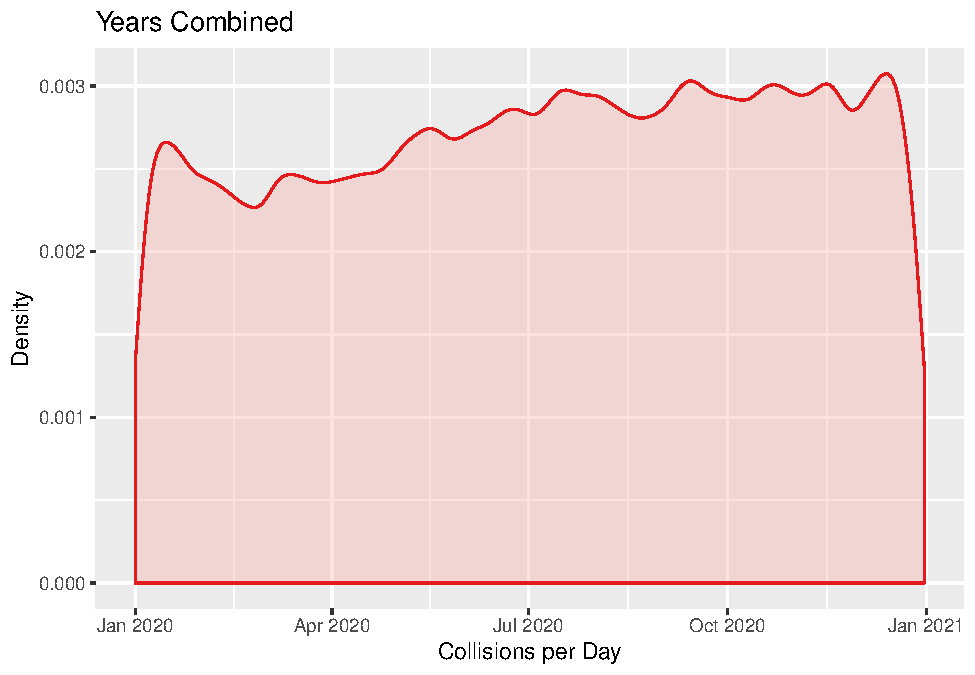
\includegraphics{RMarkdown-Group_10-Assignment_1_files/figure-latex/unnamed-chunk-6-1} 

}

\caption[Collisions per Day - Years Combined]{Collisions per Day - Years Combined}\label{fig:unnamed-chunk-6}
\end{figure}
\end{Schunk}

\hypertarget{feature-engineering}{%
\section{Feature Engineering}\label{feature-engineering}}

The business problem, in simple terms, is that the NYPD wants to deploy
their police force optimally through predicting collisions. From that
very statement, it is clear that the required fields are CRASH.DATE,
CRASH.TIME, LATITUDE, LONGITUDE and collisions. The other fields are
either redundant (borough \& zip code which are redundant to longitude
\& latitude) or not directly relevant to the problem (street names,
number of pedestrians, cyclists, motorists injured or killed. These are
ancillary and a deeper level of data and not required to solve the
problem). Depending on whether a classification model or a regression
model was used, ``Collisions'' were treated as binary (did crash happen,
Y/N?) or as a sum, respectively. Through further research, it was found
that NYPD manages NY city by Precincts. A precinct is a district of a
city or town defined for police purposes. The NYC open data website also
has data about precincts and their shape files. These shape files were
used to convert every Longitude, Latitude point into a precinct by
finding out the shape polygon in which that Longitude, Latitude point
fell. Further, for all classification models, the data was imputed with
`0' collisions data where needed, as the original data contained only
crashes.

\hypertarget{primary-data-cleaning}{%
\section{Primary Data Cleaning}\label{primary-data-cleaning}}

\hypertarget{the-problem}{%
\subsection{The Problem}\label{the-problem}}

While the Motor Vehicle Collisions -- Crashes" dataset on NYC Open Data
contains every motor vehicle collision within the City of New York,
there is a singular problem with this dataset that prevents us from
using it for the purpose of creating a supervised, binary classification
model: it only contains positive observations (i.e.~motor vehicle
crashes). Therefore, to make this dataset usable for the intended
supervision problem as stated, negative observations must be created to
complement the dataset. In addition, a binary response variable would be
created afterwards to identify the positive and negative observations.

However, the creation of negative observations itself is not a simple
problem to solve. for our motor vehicle collision dataset. Each row of
the dataset represents a specific motor vehicle collilsion at a
particular point in time, as represented by the \texttt{CRASH\ DATE} and
\texttt{CRASH\ TIME} columns, and a particular point in space, as
represented by the \texttt{LATITUDE} and \texttt{LONGITUDE} columns. For
every motor vehicle collision that has been captured by the dataset,
there are potentially thousands, or even hundreds of thousands of
collisions that did not happen at any given point in time or space. To
put into perspective, let us look at the statistics to show a rough
estimate that the likelihood of an average driver being a participant of
a car crash. For example, of the 3.8 million commuters in New York City
on a regular workday, approximately 27\% of the commuters do so by car,
truck, or van
(\url{https://edc.nyc/article/new-yorkers-and-their-cars}). Assuming
that half the commuters carpool
(\url{https://www.citylab.com/transportation/2019/01/commuting-to-work-data-car-public-transit-bike/580507/}),
and the rest drive solo, this would mean, at the very least, there are a
bit more than half a million vehicles on the road on any given workday.
Out of the half a million or so vehicles on New York City roads, there
are only about 678 car crashes in New York each day
(\url{https://www.dandalaw.com/are-car-accidents-common-in-new-york-city/},
but ideally we should calculate this from our dataset!!!). All these
numbers point out that getting into a motor vehicle collision, even in a
city with an unsafe road reputation like New York, is an unlikely event.

Consequently, to generate negative observations would yield a hugely
imblanaced dataset, consisting mostly of negative observations, and very
few positive observations. In addition, these negative observations
would also have to have generated features, such as
\texttt{CRASH\ DATE}, \texttt{CRASH\ TIME}, \texttt{LATITUDE},
\texttt{LOGITUDE}, etc. This itself is also another issue, as we cannot
randomly generate those features without understanding the distribution
of New York City traffic across different areas and times, since some
boroughs of New York, such as Staten Island, will have less traffic, and
therefore less motor vehicle accidents than other boroughs (we should
ideally show graphs of the number of accidents per borough).

\hypertarget{the-proposed-solution}{%
\subsection{The Proposed Solution}\label{the-proposed-solution}}

An easier solution to the problem of generating negative observations is
to: (a) group the positive observations by pre-determined datetime
ranges, and pre-determined geolocation areas, (b) aggregate the number
motor vehicle collisions into a column containing the counts of motor
vehicle crashes given a pre-determined datetime range, and
pre-determined geolocation area, and (c) via inference, generate
negative observations from the grouped, and aggregated positive
observations. By generalizing both the time and space of motor vehicle
collisions, the generation of negative observations will not likely
create a highly imbalnaced dataset that heavily skewers towards the
negative class, but also there is now no need to generate those features
whilst having to research the New York City traffic flow across
different space-time groups. Nevertheless, it is still important to
determine an appropriate datetime range, and geo-location areas to bin
the observations; it must be taken into account these pre-determined
datetime ranges, and geo-location areas should not only prevent extreme
class imbalance towards either positive or negative class, but also be
relevant to our business problem.

For this particular business problem, it would make sense to use New
York Police Department precincts as the pre-determined geolocation areas
group the positive observations by. This made sense given our business
problem was from a NYPD point of view, as they could divert police
resources from other precincts that are less likely to experience motor
crashes to other precincts with potentially higher collision rates. We
also experimented to use hourly bins, as we felt it would be useful for
the police to accurately predict which precinct would likely have more
motor vehicle accidents. Overall, using hourly bins and NYPD precincts
allowed the dataset to have 77\% negative observations, and roughly 23\%
positive observations, which was good enough to have only a moderate
imbalance.

\hypertarget{creation-of-the-precinct-column}{%
\subsection{Creation of the Precinct
column}\label{creation-of-the-precinct-column}}

To map the NYPD precinct, the GeoJson containing all the MultiPolygons
of NYPD precincts was downloaded from
\url{https://data.cityofnewyork.us/Public-Safety/Police-Precincts/78dh-3ptz}.
Each MultiPolygon consists of an array of Polygons, and in turn, each
Polygon consists of an array of Latitude and Longitude coordinates.
Looping through each positive observation in the dataset, the correct
precinct would be assigned to each positive observation.

As an example:

\begin{longtable}[]{@{}llll@{}}
\toprule
CRASH DATETIME & LATITUDE & LONGITUDE & PRECINCT\tabularnewline
\midrule
\endhead
06/09/2019 11:32 & 40.725210 & -73.995860 & 5\tabularnewline
06/09/2019 12:55 & 40.586680 & -73.945114 & 61\tabularnewline
06/09/2019 11:11 & 40.720626 & -73.994971 & 5\tabularnewline
\bottomrule
\end{longtable}

\hypertarget{creation-of-a-crash_binary-column}{%
\subsection{Creation of a CRASH\_BINARY
column}\label{creation-of-a-crash_binary-column}}

We then create a \texttt{CRASH\_BINARY} column for each positive
observation. All of the positive observations will have a
\texttt{CRASH\_BINARY} value of 1, denoting a positive observation.

\begin{longtable}[]{@{}lllll@{}}
\toprule
CRASH DATETIME & LATITUDE & LONGITUDE & PRECINCT &
CRASH\_BINARY\tabularnewline
\midrule
\endhead
06/09/2019 11:32 & 40.725210 & -73.995860 & 5 & 1\tabularnewline
06/09/2019 12:55 & 40.586680 & -73.945114 & 61 & 1\tabularnewline
06/09/2019 11:11 & 40.720626 & -73.994971 & 5 & 1\tabularnewline
\bottomrule
\end{longtable}

\hypertarget{round-date-time-to-nearest-hour}{%
\subsection{Round Date Time to nearest
Hour}\label{round-date-time-to-nearest-hour}}

We round the \texttt{CRASH\ DATETIME} column to the nearest hour. It is
always rounded down (i.e.~if it is 11:59AM for example, it is rounded
down to 11AM). ROUNDEDCRASH DATETIME \textbar{} LATITUDE \textbar{}
LONGITUDE \textbar{} PRECINCT \textbar{} CRASH\_BINARY \textbar{}
------------------------ \textbar{} ------------- \textbar{}
------------ \textbar{} ------------ \textbar{} ------------- \textbar{}
06/09/2019 11:00 \textbar{} 40.725210 \textbar{} -73.995860 \textbar{} 5
\textbar{} 1 \textbar{} 06/09/2019 12:00 \textbar{} 40.586680 \textbar{}
-73.945114 \textbar{} 61 \textbar{} 1 \textbar{} 06/09/2019 11:00
\textbar{} 40.720626 \textbar{} -73.994971 \textbar{} 5 \textbar{} 1
\textbar{}

\hypertarget{creation-of-negative-observations}{%
\subsection{Creation of Negative
Observations}\label{creation-of-negative-observations}}

After assigning a precinct to each positive positive observation,
negative observations must now be created. We first group the positive
obserations by \texttt{PRECINCT} and \texttt{CRASH\ DATETIME}, and
aggregate the groups by the sum by CRASH\_BINARY

\begin{longtable}[]{@{}lll@{}}
\toprule
ROUNDEDCRASH DATETIME & PRECINCT & CRASH\_BINARY SUM\tabularnewline
\midrule
\endhead
06/09/2019 11:00 & 5 & 2\tabularnewline
06/09/2019 12:00 & 61 & 1\tabularnewline
\bottomrule
\end{longtable}

We will also need to create negative observations. In this small
example, there would be no crash accidents in Precinct 61 at 11AM, and
the same could be said for Precinct 5 at 12AM. For the real dataset,
this imputation of negative observations was done for all possible
permutations of precincts (77 possible precincts) and hourly bins (24
hourly bins), but it is not shown in the example due to its length.
Therefore, for each day, there are a total of 1848 possible
observations, whether positive or negative. CRASH\_BINARY SUM for these
negative observations are assigned a numeric value of 0.

\begin{longtable}[]{@{}lll@{}}
\toprule
ROUNDEDCRASH DATETIME & PRECINCT & CRASH\_BINARY SUM\tabularnewline
\midrule
\endhead
\ldots{} & \ldots{} & \ldots{}\tabularnewline
06/09/2019 10:00 & 61 & 0\tabularnewline
06/09/2019 11:00 & 5 & 2\tabularnewline
06/09/2019 11:00 & 61 & 0\tabularnewline
06/09/2019 12:00 & 5 & 0\tabularnewline
06/09/2019 12:00 & 61 & 1\tabularnewline
06/09/2019 13:00 & 5 & 0\tabularnewline
\ldots{} & \ldots{} & \ldots{}\tabularnewline
\bottomrule
\end{longtable}

\hypertarget{split-datetime-into-month-week-day-weekday-and-hour}{%
\subsection{Split Datetime into MONTH, WEEK, DAY, WEEKDAY, and
HOUR}\label{split-datetime-into-month-week-day-weekday-and-hour}}

Lastly, for each datetime observation, the datetime was split into its
corresponding month (month of the year), week (week of the year), day
(day of the month), weekday (0 to 6, where 0 represents Monday, and 6
represents Sunday), and of course hour (in 24-hour time).

\begin{longtable}[]{@{}llllllll@{}}
\toprule
ROUNDEDCRASH DATETIME & PRECINCT & CRASH\_BINARY SUM & MONTH & WEEK &
DAY & WEEKDAY & HOUR\tabularnewline
\midrule
\endhead
\ldots{} & \ldots{} & \ldots{} & \ldots{} & \ldots{} & \ldots{} &
\ldots{} & \ldots{}\tabularnewline
06/09/2019 10:00 & 61 & 0 & 9 & 36 & 6 & 4 & 10\tabularnewline
06/09/2019 11:00 & 5 & 2 & 9 & 36 & 6 & 4 & 11\tabularnewline
06/09/2019 11:00 & 61 & 0 & 9 & 36 & 6 & 4 & 11\tabularnewline
06/09/2019 12:00 & 5 & 0 & 9 & 36 & 6 & 4 & 12\tabularnewline
06/09/2019 12:00 & 61 & 1 & 9 & 36 & 6 & 4 & 12\tabularnewline
06/09/2019 13:00 & 5 & 0 & 9 & 36 & 6 & 4 & 13\tabularnewline
\ldots{} & \ldots{} & \ldots{} & \ldots{} & \ldots{} & \ldots{} &
\ldots{} & \ldots{}\tabularnewline
\bottomrule
\end{longtable}

\hypertarget{cleaned-data-exploration}{%
\subsection{Cleaned Data Exploration}\label{cleaned-data-exploration}}

{[}TEXT ABOUT EXPLORING THE DATA{]}

\#density plot

\begin{Schunk}
\begin{figure}

{\centering \includegraphics{RMarkdown-Group_10-Assignment_1_files/figure-latex/data-exploration-1} 

}

\caption[Plots of Selected Features]{Plots of Selected Features}\label{fig:data-exploration}
\end{figure}
\end{Schunk}

\begin{Schunk}
\begin{Sinput}
#crash_dates <- as.Date(raw_crashes_data$CRASH.DATE, "%m/%d/%Y")
#ggplot(raw_crashes_data, aes(x=CRASH.DATE))
\end{Sinput}
\end{Schunk}

\hypertarget{models}{%
\section{Models}\label{models}}

As we worked through the data set, we were unsure as to which supervised
machine learning models would best suit our business needs. As such, we
have run, evaluated and compared the following 6 models:

\begin{itemize}
\tightlist
\item
  Decision Tree
\item
  Gradient Boosting
\item
  K-Nearest Neighbor
\item
  Logistic Regression
\item
  Random Forest
\item
  Regression Tree (Decision Tree Alternate Output)

  \begin{itemize}
  \tightlist
  \item
    In this model we attempted to outut \# of crashes rather than a
    binary variable for crash/no crash.
  \end{itemize}
\end{itemize}

\hypertarget{stochastic-gradient-boosting-gbm}{%
\subsection{Stochastic Gradient Boosting
(gbm)}\label{stochastic-gradient-boosting-gbm}}

Stochastic Gradient Boosting is a method of supervised learning, where
it continuously iterates over each tree one at a time to boost the
performance of its weaker learners. Unlike other types of Gradient
Boosting algorithms, Stochastic Gradient Boosting allows a base learner
to draw samples randomly from the training set. There were a few
hyperparamters to tune: \texttt{n.trees} denotes the number of trees,
\texttt{interaction.depth} denotes the maximum depth of each tree,
\texttt{n.minobsinnode} denotes the minimum number of observations in
the final node of the trees, and \texttt{shrinkage} denotes the
shrinkage, or learning rate for each tree. We used a grid search for
finding the appropriate hyperparameters for gbm, with values of 10 and
20 for \texttt{interaction.depth}, and values of 50, 100, and 250 for
\texttt{n.trees}. For the other hyperparameters, we left
\texttt{n.minobsinnode} at 10, and \texttt{shrinkage} at 0.1. We found
the gbm model performed the best, in terms of metrics, at a
\texttt{interaction.depth} of 20, and a \texttt{n.trees} of 250,
although doing so also increased the time to train the gbm model.

\hypertarget{random-forest-rf}{%
\subsection{Random Forest (rf)}\label{random-forest-rf}}

Random Forests/Decision Trees is an ensemble learning method for
classification and regression problems. Using a large number of
individual decision trees, the one with the most votes is chosen as the
prediction. There are two hyperparameters to tune: \texttt{ntree} and
\texttt{mtry}. \texttt{ntree} denotes the number of trees, whereas
\texttt{mtry} denotes the number of variables to use for splitting at
each tree node. We decided to use a \texttt{ntree} of 250, as for a
\texttt{ntree} size any larger than 250 resulted in a significantly
longer training time, and memory overflow issues. We also used a
\texttt{mtry} of 2, as this was the default and recommended number,
which was calculated based on the rounded down square root of the
cardinality of predictors
(\url{http://code.env.duke.edu/projects/mget/export/HEAD/MGET/Trunk/PythonPackage/dist/TracOnlineDocumentation/Documentation/ArcGISReference/RandomForestModel.FitToArcGISTable.html}).

\hypertarget{knn-knn}{%
\subsection{KNN (knn)}\label{knn-knn}}

K-Nearest Neighbour is a prediction algorithm used for classification
and regression problems. It works by taking each point in the dataset,
and looks at k-nearest neighbours to decide which class a particular
point belongs to. A disadvantage of KNN is that the features have to be
scaled and normalized. THis itself was not an issue for this particular
model, as all features except \texttt{Precint} were numeric. There is
only one hyperparamter to tune for KNN, which is the \texttt{k} number.
\texttt{k} denotes the nearest number of neighouring points to calculate
the Euclidean distance from. We tried a variety of \texttt{k}
parameters, ranging from 3, 5, 7, 9, and 11, but changing the \texttt{k}
parameter achieved negligble prediction improvements in our metrics.

\#\#Decision Tree

The Decision tree algorithm is a simple tree based algorithm that allows
for easy modeling and interpretation to the end business user. Though
understood to be computationally complex, the model works well in the
given context and helps identify if there will be a collision for a
given Police Precinct.

\#\#Regression Tree (Decision Tree Alternate Output) Approaching the
case as a prediction problem, leads us to consider regression
algorithms. The features in consideration aren't linearly related and
hence non parametric algorithms are used. Regression trees easily model
non linearity and avoids the assumptions of normal regression methods.
The regression tree helps determine the no.of collisions that can happen
at a given Precinct.

\hypertarget{evaluation}{%
\section{Evaluation}\label{evaluation}}

\begin{Schunk}
\begin{figure}

{\centering \includegraphics{RMarkdown-Group_10-Assignment_1_files/figure-latex/AUC-comparison-1} 

}

\caption[AUC Comparison]{AUC Comparison}\label{fig:AUC-comparison}
\end{figure}
\end{Schunk}

\hypertarget{document-style-attribution}{%
\subsection{Document Style
Attribution}\label{document-style-attribution}}

This document was generated using a modified version of the
``RJournal.sty'' file provided by the The R Foundation at
\url{https://journal.r-project.org/submissions.html}.

Inspiration, useful package suggestions and some sample code for the
xtables and ggplot functionality has been reproduced from the example
assignment 1 R Markdown file created by V2MSLabs
(\url{https://github.com/v2msLabs/ML1000-1/blob/master/source/main.Rmd}).

The document can be regenerated in RStudio by Knitting the provided ``R
Markdown-Group 10-Assignment 1.Rmd'' file with the provided
``RJournal.sty'' file in the same directory.

\hypertarget{default-r-markdown-code-below}{%
\section{DEFAULT R MARKDOWN CODE
BELOW}\label{default-r-markdown-code-below}}

\hypertarget{r-markdown}{%
\subsection{R Markdown}\label{r-markdown}}

This is an R Markdown document. Markdown is a simple formatting syntax
for authoring HTML, PDF, and MS Word documents. For more details on
using R Markdown see \url{http://rmarkdown.rstudio.com}.

When you click the \textbf{Knit} button a document will be generated
that includes both content as well as the output of any embedded R code
chunks within the document. You can embed an R code chunk like this:

\begin{Schunk}
\begin{Sinput}
summary(cars)
\end{Sinput}
\begin{Soutput}
#>      speed           dist       
#>  Min.   : 4.0   Min.   :  2.00  
#>  1st Qu.:12.0   1st Qu.: 26.00  
#>  Median :15.0   Median : 36.00  
#>  Mean   :15.4   Mean   : 42.98  
#>  3rd Qu.:19.0   3rd Qu.: 56.00  
#>  Max.   :25.0   Max.   :120.00
\end{Soutput}
\end{Schunk}

\hypertarget{including-plots}{%
\subsection{Including Plots}\label{including-plots}}

You can also embed plots, for example:

\begin{Schunk}

\includegraphics{RMarkdown-Group_10-Assignment_1_files/figure-latex/pressure-1} \end{Schunk}

Note that the \texttt{echo\ =\ FALSE} parameter was added to the code
chunk to prevent printing of the R code that generated the plot.


\address{%
Alex Fung\\
\\
\\
}


\address{%
Viswesh Krishnamurthy\\
\\
\\
}


\address{%
Tony Lee\\
\\
\\
}


\address{%
Patrick Osborne\\
\\
\\
}


